\section{复习}
\courseTime{Sep. 26, 2022\\Week 4}
%2022-09-26 07:59:45  Wenbin Fan @FDU 
\chat{%
早上好。人少了一点,我们都是选了这课的。

第一次课回顾了量子力学的诞生,我们想从量子力学初期实验现象演绎出薛定谔方程。其中最重要的现象是波粒二象性。光波的波动方程是两个二阶偏导呈线性,薛定谔方程是二阶偏导、一阶偏导有线性关系。}

如果势函数 $V$ 与时间无关,那么则可以分离时间和坐标,对于仅包含坐标的方程为定态薛定谔方程。% 如果是自由粒子

2021 年,\emph{Science} 发布了《125 个问题:发现与发现》,其中 ``What is quantum uncertainty and why is it important?'' 是其中一个问题。\footnote{\url{https://www.science.org/content/resource/125-questions-exploration-and-discovery}}目前的量子计算、量子测量是热门领域。
\extraInfo{什么是量子不确定性,为什么它很重要?}{
海森堡不确定性原理是量子力学的一个关键原则,它指出我们不能同时测量一个物体的速度和位置。天文学家和科学记者Ethan Siegel写道:``你越是精确地测量一个物体的位置,你对其动量的了解就越是内在不准确。这不仅仅是我们仪器的失败,这种不确定性是宇宙的根本。''不确定性在量子计算中起着重要作用,它依靠电子叠加来存储信息。但是量子叠加是很棘手的事情。当你试图测量它们时,或者甚至通过与环境的共同作用,如遇到随机的电磁辐射脉冲,它们会坍缩(用量子术语)。
}

\chat{%
我们讲过了高斯波包。通过高斯波包一阶、二阶偏导之间的关联,我们演绎出了薛定谔方程,并且演绎出了光波可以回到麦克斯韦的波动方程。对于质量不为零的粒子,利用德布罗意物质波、波矢与角频率是二次关系,推出了薛定谔方程。
}

上次课讲了量子力学的公设,算符的定义。

1. 微观体系都需要波函数描述

2. 可观测量对应于线性 Hermite 算符。坐标、势函数的算符就是本身。 能量与动量的关系,$E = mc, p = h/\lambda$,加上薛定谔方程可推导出$\hat p = -\ii \hbar \frac{\partial}{\partial x}$

3. $\AA f = \lambda f$ 本征方程

4. 线性 Hermite 算符的本征函数 $\{\left|\phi_i\right\rangle\}$ 构成完备集,相同坐标空间和时间空间的系统内的任何一个粒子状态都可以表示成线性算符本征值的线性展开 $\ket{\psi} = \sum_i c_i \ket{\phi_i}$,由此就有关于测量的一些讨论。

\chat{%
下周放掉一节课,我们尽量讲两节课的内容。很多结论会直接给大家。
}

\chapter{粒子的平动}

\section{一维自由粒子}

势函数为 0,定态薛定谔方程
\begin{eqnarray}
    -\frac{\hbar}{2m} \frac{\partial}{\partial x^2}\psi(x) = E \psi(x),
\end{eqnarray}
设波函数 $\psi(x) = \ee^{s x}$,得到
\begin{eqnarray}
    s = \pm \frac{\ii}{\hbar} \sqrt{2m |E|}
\end{eqnarray}
利用德布罗意关系 $E = p^2 / 2m, p = \hbar k$,推出
\begin{eqnarray}
    E = \frac{\hbar^2k^2}{2m},
\end{eqnarray}
则
\begin{eqnarray}
    s = \pm \frac{\ii}{\hbar}|p| = \pm \ii |k| = \ii k,
\end{eqnarray}
正负号表示方向,所以正向波矢自身为正,前面符号也为正,故脱掉了绝对值符号,那么波函数为
\begin{eqnarray}
    \psi(x) = \ee^{\ii kx},
\end{eqnarray}
与负方向的波函数构成通解为
\begin{eqnarray}
    \psi(x) = C_1 \ee^{\ii kx} + C_2 \ee^{-\ii kx}
\end{eqnarray}
表示向右和向左传播的波。利用欧拉公式 $\ee^{\ii\theta} = \cos\theta + \ii\sin\theta$,展开为
\begin{eqnarray}
    \psi(x) = (C_1 + C_2) \cos kx + \ii (C_1 - C_2) \sin kx.  
\end{eqnarray}
\begin{lstlisting}
Subscript[C, 1] Exp[I k x] + 
  Subscript[C, 2] Exp[-I k x] // ExpToTrig
>> Cos[k x] Subscript[C, 1] + I Sin[k x] Subscript[C, 1] + 
 Cos[k x] Subscript[C, 2] - I Sin[k x] Subscript[C, 2]
\end{lstlisting}

\subsection{流密度}
\chat{%
流密度是说密度跟概率随时间流动的速度,对应着速度的概念。
}

回忆第一节课,我们讲到量子力学公设时提到,
状态波函数必须是正交归一的,意味着演化过程中的归一性质是不变的,使得
\begin{eqnarray}
    \int_{-\infty}^\infty |\psi(x,t)|^2 \dd x = 1
\end{eqnarray}
$\psi$ 归一化是不会随时间演化而破坏的,需要满足
\begin{eqnarray}
    \frac{\partial}{\partial t} \int_{\infty}^\infty |\psi|^2 \dd x = 0
\end{eqnarray}
概率必然大于零,可以将偏导放进去,
\begin{eqnarray}
    \int_{\infty}^\infty \frac{\partial}{\partial t}  |\psi|^2 \dd x = 0
\end{eqnarray}
有
\begin{eqnarray}
    \frac{\partial}{\partial t} |\psi|^2 = \frac{\partial}{\partial t} \psi^* \psi = \frac{\partial \psi^*}{\partial t}\psi + \psi^* \frac{\partial \psi}{\partial t}
\end{eqnarray}
代入薛定谔方程
\begin{eqnarray}
    \ii\hbar \frac{\partial}{\partial t} \psi = \left[
        -\frac{\hbar^2}{2m} \frac{\partial^2}{\partial x^2} + V(x,t)
    \right]
    \psi(x,t)
\end{eqnarray}
得到
\begin{eqnarray}
    \frac{\partial}{\partial t} |\psi|^2 = \frac{\ii\hbar}{2m} \frac{\partial}{\partial x}
    \left[
        \psi^* \frac{\partial \psi}{\partial x} - \psi \frac{\partial \psi^*}{\partial x}
    \right]
\end{eqnarray}
这是个很重要的式子,在哥本哈根诠释中,$|\psi|^2 = \rho(x,t)$ 是密度,所以粒子密度随时间的演化可以表示为
\begin{eqnarray}
    \pdv{t} \rho(x,t) = \pdv{x} \left[
        \frac{\ii\hbar}{2m} \left(
            \psi^* \pdv{\psi}x - \psi\pdv{\psi^*}x
        \right)
    \right]
\end{eqnarray}
对时间的偏导等于对坐标的偏导。流体力学中连续性方程
\begin{eqnarray}
    \frac{\partial \rho}{\partial t} + \frac{\partial J}{\partial x} = 0, 
\end{eqnarray}
其中流密度为
\begin{eqnarray}
    J = -\frac{\ii\hbar}{2m} \left( \psi^* \frac{\partial \psi}{\partial x} - \psi \frac{\partial \psi^*}{\partial x}\right)
\end{eqnarray}
应用高斯定理,可得连续性方程的积分形式
\begin{eqnarray}
    \underbrace{\frac{\partial}{\partial t} \underbrace{\int_V \rho \dd^3x}_{\substack{\text{粒子在体积} \\ \text{$V$ 中的概率}}} }_{\substack{\text{粒子流入或流出}\\ \text{体积 $V$ 的速度}}} 
     + 
    \underbrace{\oint_S \underbrace{J}_{\substack{\text{粒子流入或流出}\\ \text{体积 $V$ 的通量}}} \dd a}_{\text{围绕体积 V 的面积分}} = 0,
\end{eqnarray}
如果能够满足这个偏微分方程的平衡连续方程,该方程给出 $J$ 的定义就对应于粒子流入或流出某区域的速度。当体积固定、面积变大,速度的通量就变小了。这里的 $J$ 便是流密度。

对 $J$ 简单演绎,
\begin{align}
    J &= -\frac{\ii\hbar}{2m} \left( \psi^* \frac{\partial \psi}{\partial x} - \psi \frac{\partial \psi^*}{\partial x}\right) \\
    &= \frac{1}{2m} \left[
        \psi^* \left(-\ii\hbar\frac{\partial}{\partial x}\right) \psi +
        \psi \left(-\ii\hbar\frac{\partial}{\partial x} \psi\right)^*
    \right] \\
    &= \frac1{2m} \left[\psi^* \hat p \psi + (\hat p\psi)^* \psi\right]
\end{align}
因此,描述粒子运动的流密度可以由动量算符构造出来。

代入自由粒子的状态方程,
\begin{eqnarray}
    \psi(x,t) = a \exp (\ii k x) \exp \left( - \frac{\ii\hbar^2k^2}{2m}t\right), \quad k\hbar = p = mv,
\end{eqnarray}
%2022-09-26 08:33:07  Wenbin Fan @FDU
有
\begin{eqnarray}
    J = -\frac{\ii\hbar}{2m} [|a|^2 \ii k + |a|^2 \ii k] = \frac{\hbar k} m |a|^2 = |a|^2 v
\end{eqnarray}
流密度与速度成正比,可将 $J$ 看成粒子的运动速度。

\chat{%
可观测量对应的都是 Hermite 线性算符。某算符 $\AA$ 的期望值为,作用到状态波函数上并全空间积分,当且仅当状态函数为算符的本征函数时,算符作用上去得到本征值和本征函数。那么 $J$ 也应该当作算符,但是为什么没有?因为恰好自由粒子时动量函数的本征函数,所以全空间积分是一样的。

但是我们遇到了归一化问题。
}

\subsection{归一化问题}
一维自由粒子波函数的模方
\begin{eqnarray}
    \int_{-\infty}^\infty \psi^*\psi \dd x = |a|^2 \int_{-\infty}^\infty \dd x
\end{eqnarray}
显然是不可归一化的。
\chat{%
按照量子力学公设第一条,品优波函数描述微观粒子性质,但这里不能归一。所以结论是,不存在处于定态(给定 $k$)的自由粒子。
这里有些简单粗暴了,我们算出来是这个微观状态,但因为不能归一所以就断言不存在这样的状态。

对光而言,它没有初始状态,可以描述成这个状态。对粒子而言,波是内禀属性,不意味着静止的时候可以离散到全空间。我们推过光波的波包,随时间演化永远不会发散的。粒子的波包随时间弥散,这是不对的。
}

但是,不处于定态的自由粒子并非不可描述。自由粒子的定态波函数是动能算符 $\hat T$ 的本征函数,
\begin{eqnarray}
    \left\{\psi(x,t) = a \exp (\ii k x) \exp \left( - \frac{\ii\hbar^2k^2}{2m}t\right)
    \right\},
\end{eqnarray}
因为 $\hat T$ 是 Hermite 算符,所以构成完备集。任何一个粒子,不处于定态,就可以展开成全空间求和
\begin{eqnarray}
    \psi_0 (x,t) = \sum_k c_k\psi_k(x,t) = \int_{-\infty}^\infty c_k\psi_k (x,t) \dd k = \int_{-\infty}^\infty A(k) \psi_k(x,t) \dd k, \label{eq:wave_expand_fullSet}
\end{eqnarray}
表示成波包的样子。

\chat{%
这里有很多个人看法,不见得完全正确。我能保证最终结论是对的,保证数学推导肯定不错,但中间阐述是见仁见智的问题。本来量子力学背后就有很多种不同的解释。

假设一个粒子,我们准备好了它的初态,再也不给它任何的束缚,那么该粒子的演化一定遵循薛定谔方程。
}
%2022-09-26 08:44:08  Wenbin Fan @FDU

% 休息
% 第二节课 % 2022-09-26 08:53:53  Wenbin Fan @FDU

准备初态,
在实空间的表示形式
\begin{eqnarray}
    \psi(x,0) = \frac{1}{\sqrt{2\pi}} \intinf A(k) \ee^{\ii kx} \dd x, 
\end{eqnarray}
利用反 Fourier 变换关系,得到微观粒子处在第 $k$ 个态的概率,也就是在 $k$ 空间(动量空间)的概率分布,
\begin{eqnarray}
    A(k) = \frac{1}{\sqrt{2\pi}} \intinf \psi(x,0) \ee^{\ii kx} \dd x,
\end{eqnarray}
结合量子力学公设第四条,任何波函数都可以由另外一组波函数线性展开。

%2022-09-26 08:58:34  Wenbin Fan @FDU
构造一个自由粒子的初态,
\begin{eqnarray}
    \psi(x,0) = 
    \begin{cases}
        \frac1{\sqrt{2a}},\quad &x\in[-a,a],\\
        0, \quad &\text{其它}
    \end{cases}
\end{eqnarray}
这是一个阶梯函数,积分得到
\begin{eqnarray}
    A(k) = \frac1{\sqrt{2a}} \frac{\sin ak}{k}
\end{eqnarray}
在 $k$ 空间却是一个全空间的正弦函数,这在通讯领域中的数模转换时常用。
有了 $A(k)$ 之后可以用来构造波函数,参考式子 \eqref{eq:wave_expand_fullSet}
\begin{eqnarray}
    \psi(x,t) = \frac1{\sqrt{2\pi}} \intinf A(k,t) \ee^{\ii k x} \dd k. 
\end{eqnarray}

讨论 (1) 如果 $a$ 很小,束缚在很窄的一个范围内,那么
\begin{eqnarray}
    A(k) = \frac{1}{\pi a} \frac{\sin ak}{k} \approx \frac{\sqrt{a}}{\sqrt\pi}
\end{eqnarray}
与 $k$ 无关,表示动量展宽很大、不确定,位置确定

(2) 如果 $a$ 很大,
\begin{eqnarray}
    A(k) = \sqrt{\frac{a}{\pi}} \frac{\sin ak}{ak}
\end{eqnarray}
当 $k\rightarrow 0$ 时,$A(k)$ 取极大值,即 $|A(k)|^2$ 取极大值。此时位置不确定,动量确定。

\homework{
    \textbf{3.1}  对于给出下述初态 $\psi(x,t=0)$,即初始时刻自由粒子($V(x) = 0$)波函数,求出 $\psi(x,t)$ 含时演化波函数,其中 $a>0, b\in\mathbb{R}, x\in\mathbb{R}$,

    (a) $A \ee^{-a|x|}$, (b) $A\ee^{-ax^2}$, (c) $A \ee^{-ax^2} \ee^{-\ii b x}$. 
}

% 2022-09-26 09:09:14  Wenbin Fan @FDU
\section{一维势箱中的粒子}
\begin{figure}[tp]\centering
    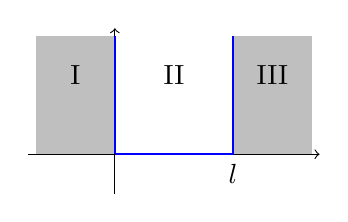
\begin{tikzpicture}[scale=0.5]
        % region
        \fill[lightgray] (-2,0) rectangle (0,3);
        \fill[lightgray] (3,0) rectangle (5,3);
        % axis
        \draw[->] (-2.2,0) -- (5.2, 0);
        \draw[->] (0,-1) -- (0, 3.2);
        % potential
        \draw[thick,blue] (0,0) -- (3,0);
        \draw[thick,blue] (0,0) -- (0,3);
        \draw[thick,blue] (3,0) -- (3,3); 
        % text
        \node[] at (-1,2) {I};
        \node[] at (1.5,2) {II};
        \node[] at (4,2) {III};
        
        \node[below] at (3,0) {$l$};
        % functions
        % \draw[domain=-4:4,black,thick,samples=100] plot (\x,{\x*\x});
    \end{tikzpicture}
    \caption{无限深势阱}
    \label{fig:inf_well}
\end{figure}
微观体系都是由品优波函数描述。
不管如何,先写出薛定谔方程。
\begin{eqnarray}
    \hat H \psi = (\hat T + V) \psi = E \psi,
\end{eqnarray}
势能函数
\begin{eqnarray}
    V(x) =
    \begin{cases}
        0, \quad &x\in [0,l]\\
        \infty, \quad &\text{其它}
    \end{cases}
\end{eqnarray}
薛定谔方程写为
\begin{align}
    (V-E) \psi &= \frac{\hbar^2}{2m} \pdv[2]{x} \psi \\
    \psi &= \frac{\hbar^2}{2m(V-E)} \pdv[2]{x} \psi,
\end{align}
对于 block I 和 III,$\psi(x) = 0$,对于 block II 有 
\begin{eqnarray}
    \psi(x) = C_1 \ee^{\ii k x} + C_2 \ee^{-\ii k x} = A \cos kx + B \sin kx,
\end{eqnarray}
这个解是普适的,导致体系量子化的是\boldtext{边界条件}。
%2022-09-26 09:15:15  Wenbin Fan @FDU
由边界条件来约束系统呈现出的状态,否则通解没有使用价值。

根据品优波函数的要求,波函数必须连续,
\begin{eqnarray}
    \psi(0) = \psi(l) = 0,
\end{eqnarray}
在 $x=0$ 处有
\begin{eqnarray}
    \psi(0) = A \cos 0 + B \sin 0 = 0,
\end{eqnarray}
立刻可得 $A = 0$,波函数为 $\psi(x) = B \sin kx$。在 $x=l$ 处,
\begin{eqnarray}
    \psi(l) = B \sin kl = 0,
\end{eqnarray}
得到量子化条件
\begin{eqnarray}
    k l = n \pi \rightarrow k = \frac{n\pi}{l}
\end{eqnarray}
其中 $n$ 为整数,所以该体系是量子化的。当 $n=0$ 时,舍去。由于 $n$ 为负时与 $n$ 为正时一样,没有新的物理,故令 $n \in \mathbb{N}^+$。得到解
\begin{eqnarray}
    \psi_n(x) = 
    \begin{cases}
        B \sin \frac{n\pi x}l, \quad &x \in [0,l], n\in\mathbb{N}^+, \\
        0,\quad &\text{其它}
    \end{cases}
\end{eqnarray}
% 【讨论为何只需要原函数连续,不需要高阶连续】【录音 1h 26min】
% 【n=0 为啥要舍去?补充】

\subsection{一维势箱的性质}

(1) 归一化 $\left\langle \psi_n \middle | \psi_n \right\rangle = 1$, 即
\begin{align}
    &= B^2 \int_0^l \sin^2 \frac{n\pi x}{l} \dd x \\
    &=  B^2 \int_0^l \left[\cos 0 - \cos \frac{2 n \pi x}l \right] \dd x \\
    &= \frac l2 B^2 + 0 = 1
\end{align}
其中利用了三角函数的变换
\begin{eqnarray}
    2\sin\alpha \sin\beta = \cos(\alpha-\beta) - \cos(\alpha+\beta),
\end{eqnarray}
因此,归一化条件为 $B = \pm \sqrt{\frac2l}$,波函数重写为
\begin{equation}
    \phi_n(x) = \begin{cases}\displaystyle
        \sqrt{\frac 2l} \sin\frac{n\pi x}l, \quad &x\in[0,l], n\in \mathbb{N}^+,\\
        0, \quad&\text{其它},
    \end{cases}
\end{equation}
注意到,归一化条件只与 $l$ 有关,与量子数 $n$ 无关。
\begin{lstlisting}
(* 画出一维势阱的波函数,n=0,...,5 *)
l = 1; (* 宽度 *)
Plot[Table[Sqrt[2/l] Sin[(n \[Pi] x)/l], {n, 0, 5}] // Evaluate, {x, 0, l}, Filling -> Axis]
\end{lstlisting}

(2) 不同量子数的波函数之间正交

当 $m \neq n$ 时,
\begin{align}
    \left\langle \psi_n \middle | \psi_n \right\rangle 
    &= \intinf \psi_n^* (x) \psi_m(x) \dd x \\
    &= \frac2l \int_0^l \sin \frac{n\pi x}{l} \sin \frac{n\pi m }{l} \dd x, \\
    &= \frac 1l \int_0^l \left[
        \cos \frac{(n-m)\pi x}l - \cos\frac{(n+m)\pi x}l
    \right] \dd x \\
    &= 0
\end{align}
因此波函数之间均满足正交归一,
\begin{eqnarray}
    \left\langle \psi_n \middle | \psi_n \right\rangle = \delta_{mn} = \begin{cases}
        1, \quad &m=n,\\
        0, \quad &m\neq n,
    \end{cases}
\end{eqnarray}

(3) 动量算符的平均值为 0
\begin{align}
    \ev{\hat p} 
    &= \left\langle \psi_n \middle| \hat p \middle| \psi_n \right\rangle \\
    &= - \ii \hbar \int_0^l \cos\frac{n \pi x}l \frac{\partial}{\partial x} \cos \frac{n\pi x}l \dd x \\
    &= \ii\hbar \frac{n\pi}l \int_0^l \cos \frac{n\pi x}l \sin\frac{n\pi x}l \dd x \\
    &= \frac{\ii\hbar}2 \frac{n\pi}l \int_0^l \left(\sin\frac{2n\pi x}{l} - \sin 0\right)\dd x \\
    &= \frac{\ii\hbar}2 \frac{n\pi}l \left(- \cos \frac{2n\pi x}l\right) \bigg|_0^l = 0,  
\end{align}
\begin{lstlisting}
Clear["Global`*"]
res = Integrate[
    Cos[(n \[Pi] x)/l] (-I \[HBar]) D[Cos[(n Pi x)/l], x], {x, 0, l}]
Simplify[res, Assumptions -> {n \[Element] Integers}]
>> 1/2 I \[HBar] Sin[n \[Pi]]^2
>> 0
\end{lstlisting}
其中利用了积化和差
\begin{equation}
    \sin\alpha \, \cos\beta = \frac12 \sin(\alpha+\beta) + \frac12 \sin(\alpha-\beta),
\end{equation}
所以流密度算符的平均值也为 0。

(4) 动量绝对值的平均值不为 0

首先求出动量平方的平均值,
\begin{align}
    \ev{\hat p^2} &= \langle \psi_n | \hat p^2 | \psi_m \rangle \\
    &= \frac{n^2\pi^2\hbar^2}{l^2} = \frac{n^2h^2}{l^2}
\end{align}
所以动量绝对值的平均值为
\begin{align}
    \rightarrow |p| = \sqrt{\ev{\hat p^2}} = \frac{n\hbar}{2l},
\end{align}
\begin{lstlisting}
res = 
Integrate[
    Sqrt[2/l] Cos[(n \[Pi] x)/l] (-I \[HBar])^2 D[
    Sqrt[2/l] Cos[(n Pi x)/l], {x, 2}], {x, 0, l}]
Simplify[res, 
    Assumptions -> {n \[Element] Integers}] /. {\[HBar] -> h/(2 Pi)}
>> (n \[Pi] \[HBar]^2 (2 n \[Pi] + Sin[2 n \[Pi]]))/(2 l^2)
>> (h^2 n^2)/(4 l^2)
\end{lstlisting}
即物质波长 $|p| = \frac{h}{\lambda}$, 得到 $\lambda = \frac h{|p|} = \frac{2l}n$。 

\extraInfo{不确定关系}{
    求出以下算符的平均值,
    \begin{align}
        &\ev{x} = \frac l2, \quad \ev{x^2} = \frac{1}{6} l^2 \left(\frac{3}{\pi^2 n^2}+2\right), \\
        &\ev{p} = 0, \quad \ev{p^2} = \left(\frac{n \pi\hbar}l\right)^2,
    \end{align}
    因此坐标和动量的涨落为
    \begin{align}
        &\sigma_p^2 = \ev{p^2} - \ev{p}^2 = \left(\frac{n \pi\hbar}l\right)^2, \\
        &\sigma_x^2 = \ev{x^2} - \ev{x}^2 = \frac{l^2}2 \left( \frac16 + \frac1{n^2\pi^2} \right),
    \end{align}
    所以不确定关系
    \begin{align}
        \Delta x \Delta p = \frac{\hbar}2 \sqrt{2+\frac{n^2\pi^2}3 } \ge \frac{\hbar}2
    \end{align}
    得到了验证。
}

(5) 能量的平均值

直接利用前面求解出的动量平方的平均值,有
\begin{align}
    E_n = \langle \hat T \rangle = \frac1{2m} \ev{\hat p^2} = 
    \frac{n^2h^2}{8ml^2}
\end{align}

(a) 由于 $n=0$ 不被允许,$E_1 = \frac{h^2}{8ml^2}$ 为\boldtext{零点能},

(b) 能级差
\begin{align}
    \Delta E_n = E_{n+1} - E_n = (2n+1) \frac{h^2}{8ml^2}
\end{align}
逐渐增大,表示能量不连续的情况越来越严重,这偏离了从量子到经典变化的过程。


(6) 粒子密度分布
\begin{eqnarray}
    \rho(x) = |\psi(x)|^2 = \frac 2l \sin^2 \frac{n\pi x}l, x\in[0,l]
\end{eqnarray}
波函数在区间 $(0,l)$ 中存在 $n-1$ 个节点,节点即 $\psi(x) = 0$ 的位置。观察易知,波函数的最大曲率与量子数 $n$ 有关,因此量子数越大,最大曲率也会越大。
\begin{lstlisting}
(* 粒子密度 *)
l = 1;
Plot[Table[2/l Sin[(n \[Pi] x)/l]^2, {n, 1, 5}] // Evaluate, {x, 0, 
  l}, Filling -> Axis]
\end{lstlisting}
当量子数趋于无穷,物质波波长越来越短,行为越像粒子,但是对于当前体系的波函数并不是这样。考察
\begin{eqnarray}
    \frac{\Delta E}{E} = \frac{2n+1}{n^2} \rightarrow 0
\end{eqnarray}
虽然能级差越来越大,但是能级差相对于总能量的比例是越来越小的。从另一个角度来说,当 $l$ 增大的时候,波函数会变得越来越扁长。

因此,从量子过渡到经典有两个判断标准。一是当量子数趋于无穷大时,波函数行为是否从离散变连续,是否有更多波的性质。二是当微观体系的尺寸变成宏观时,波函数的变化情况。

%2022-09-26 13:10:38  Wenbin Fan @FDU
% 下午课
%2022-09-26 13:26:28  Wenbin Fan @FDU
\homework{
    \textbf{3.2} (a) 一个 \SI{100}{\gram} 的实心球限制在 \SI{5}{\metre} 的线道上,(b) 束缚在 \SI{10E-10}{\metre} 区域内的电子。求以上两种情况的零点能。

    \textbf{3.3} 讨论如下定义的势箱中的粒子,
    \begin{equation}
        V(x) = 
\begin{cases}
    0, \quad &x\in \left[-\frac l2, \frac l2\right],\\
    +\infty, \quad &\text{其它},
\end{cases}
    \end{equation}
}

合并两次课的内容。都是一维薛定谔方程,势能都是 0 或无穷大。无限深势阱是束缚态。

% \subsection{一维势箱的应用}

%3.
\section{单侧有限深势阱}
\begin{figure}[tp]\centering
    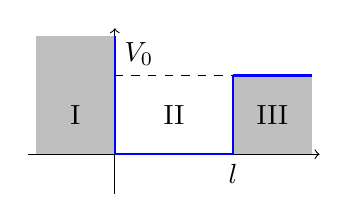
\begin{tikzpicture}[scale=0.5]
        % region
        \fill[lightgray] (-2,0) rectangle (0,3);
        \fill[lightgray] (3,0) rectangle (5,2);
        % axis
        \draw[->] (-2.2,0) -- (5.2, 0);
        \draw[->] (0,-1) -- (0, 3.2);
        % potential
        \draw[thick,blue] (0,0) -- (3,0);
        \draw[thick,blue] (0,0) -- (0,3);
        \draw[thick,blue] (3,0) -- (3,2); 
        \draw[thick,blue] (3,2) -- (5,2); 
        \draw[dashed] (0,2) -- (3,2);
        % text
        \node[] at (-1,1) {I};
        \node[] at (1.5,1) {II};
        \node[] at (4,1) {III};
    
        \node[below] at (3,0) {$l$};
        \node[above right ] at (0,2) {$V_0$};
        % functions
        % \draw[domain=-4:4,black,thick,samples=100] plot (\x,{\x*\x});
    \end{tikzpicture}
    \caption{半无限深势阱}
    \label{fig:half_inf_well}
    \end{figure}
先写出薛定谔方程
\begin{equation}
    \hat H = \hat T + \hat V(x),
\end{equation}
势能依然是分段函数,
\begin{equation}
    V(x) = 
    \begin{cases}
        +\infty, \quad &x\in(-\infty, 0),\\
        0, \quad &x\in[0,l],\\
        V_0, \quad &x\in(l,\infty),
    \end{cases}
\end{equation}

对于 block I,有
\begin{align}
    (V - E)\psi(x) &= \frac{\hbar^2}{2m} \frac{\partial \psi^2(x)}{\partial x^2} \\
    \psi(x) &= \frac{\hbar^2}{2m(V - E)} \frac{\partial^2 \psi(x)}{\partial x^2} = 0
\end{align}

对于 block II, 有
\begin{align}
    -\frac{\hbar^2}{2m} \pdv[2]{x} \psi(x) = E\psi(x),
    \label{eq:half_inf_block2_seq}
\end{align}
其通解为
\begin{equation}
    \psi(x) = C_1 \ee^{\ii k_{2}x} + C_2 \ee^{-\ii k_2 x}
\end{equation}
对应两个方向不同的波,由此引入了三个参数 $\{C_1, C_2, k_2\}$。将通解代入薛定谔方程 \eqref{eq:half_inf_block2_seq},解得 $k_2$ 与能量有关,
\begin{equation}
    E = \frac{\hbar^2}{2m} k_2^2 \rightarrow k_2 = \frac{\sqrt{2mE}}{\hbar},
\end{equation}

还是利用边界条件,求出待定参数。所有边条件都是跟品优波函数性质相关。

\textbf{边界条件 1},
\begin{equation}
    \psi(0^-) = \psi(0^+) = 0,
\end{equation}
容易得到
\begin{equation}
    C_1 \ee^0 + C_2 \ee^0 = 0,
\end{equation}
即
\begin{equation}
    C_2 = - C_1,
\end{equation}
由此将待定参数消掉一个。

对于 block III,
\begin{align}
    - \frac{\hbar^2}{2m} \pdv[2]{\psi(x)}{x} + V_0 \psi(x) &= E\psi(x), \\
    (V_0 - E) \psi(x)&= \frac{\hbar^2}{2m} \pdv[2]{x} \psi{x}
\end{align}
设 $\psi(x) = \ee^{sx}$,代回有
\begin{align}
    (V_0-E) \psi(x) &= \frac{s^2\hbar^2}{2m} \psi(x)
\end{align}
得到
\begin{eqnarray}
    s^2 = \frac{2m(V_0 - E)}{\hbar^2},
\end{eqnarray}
其中 $V_0 - E$ 的正负对结果有着决定性的影响。

当 $V_0 > E$ 时,称为\boldtext{束缚态},有
\begin{eqnarray}
    s = \pm k_3, \quad k_3 = \frac{\sqrt{2m(V_0 - E)}}{\hbar}, 
\end{eqnarray}
解得
\begin{eqnarray}
    \psi(x) = C_3 \ee^{k_3 x} + C_4 \ee^{-k_3 x},
    \label{eq:half_inf_block3_wf1}
\end{eqnarray}
%2022-09-26 13:47:16  Wenbin Fan @FDU
这时的未知参数有 $\{E, C_1, C_3, C_4\}$,其中 $E$ 是横跨三个 block 的变量,决定了 $k_2$ 和 $k_3$。接下来是一样的步骤,只要是可以精确求解的体系,比如稍复杂的氢原子,即不断引入边界条件,获得量子化的结果。

在 block I 负无穷($x=-\infty$),波函数一定为 0。在 block III 正无穷的区域,波函数一定会衰减为有限值,甚至是趋于 0 的,所以假定它不为无穷大。

\textbf{边界条件 2},
\begin{eqnarray}
    \psi(+\infty) = 0 
\end{eqnarray}
代入 \eqref{eq:half_inf_block3_wf1} 消掉了 $C_3$,还有三个待定参数 $\{E, C_1, C_4\}$。

\textbf{边界条件 3},在波函数 $x = l$ 的地方,左右波函数相等,
% 【引用 block II \& III 的波函数】
\begin{eqnarray}
    \psi(l^-) = \psi(l^+),
\end{eqnarray}
得到
\begin{eqnarray}
    C_1 \ee^{\ii k_2 l} - C_1 \ee^{-\ii k_2 l} = C_4 \ee^{-k_3 l}, \label{eq:half_condition_3}
\end{eqnarray}
还有两个待定参数。

边界条件 4,在 $x=l$ 的地方,左右波函数对坐标的偏导相等,
\begin{eqnarray}
    C_1 \ii k_2 \left[
        \ee^{\ii k_2 l} + \ee^{-\ii k_2 l} 
    \right] = - C_4 k_3 \ee^{-k_3 l} \label{eq:half_condition_4}
\end{eqnarray}
目前只剩能量 $E$ 待求。

依然使用欧拉方程,将 \eqref{eq:half_condition_3} \eqref{eq:half_condition_4} 展开成
\begin{align}
    & 2\ii \,C_1 \sin k_2l = C_4 \ee^{-k_3 l}, \\
    & 2 k_2 \ii \, C_1 \cos k_2 l = - C_4 k_3 \ee^{-k_3 l}, 
\end{align}
% [讨论为什么这么化简]
%2022-09-26 13:58:01  Wenbin Fan @FDU
左右两边分别相除
\begin{eqnarray}
    \frac1{k_2} \tan k_2l = - \frac1{k_3}. 
    \label{eq:half_inf_k2k3_0}
\end{eqnarray}
直接得到了 $k_2$ 和 $k_3$ 的关系,这样比较简单。如果分别求出 $C_1, C_4$ 和 $k_2, k_3$ 的关系,也可以讨论。

考虑到
\begin{eqnarray}
    k_2 = \frac{\sqrt{2mE}}{\hbar}, \quad k_3 = \frac{\sqrt{2m(V_0- E)}}{\hbar}, \label{eq:half_inf_k2k3_def}
\end{eqnarray}
代回 \eqref{eq:half_inf_k2k3_0},则得到能量相关的式子
\begin{eqnarray}
    \frac{\hbar}{\sqrt{2mE}} \tan \left(
        \frac l{\hbar} \sqrt{2mE}
    \right)
    = - \frac{\hbar}{2m(V_0 - E)},
    \label{eq:half_inf_k2k3_transcendental}
\end{eqnarray}
这是关于 $E$ 的超越方程,有数值解。

化简 \eqref{eq:half_inf_k2k3_transcendental},以便讨论。设
\begin{eqnarray}
    z = \frac{l}{\hbar} \sqrt{2mE}, \quad z_0 = \frac {l}{\hbar} \sqrt{2m V_0},\label{eq:half_inf_zz0_def}
\end{eqnarray}
可得
\begin{align}
    z_0^2 - z^2 &= \frac{l^2}{\hbar^2} 2m (V_0 - E),\\
    \sqrt{z_0^2 - z^2} &= \frac{l}{\hbar} \sqrt{2m (V_0 - E)},
\end{align}
所以 \eqref{eq:half_inf_k2k3_transcendental} 为
\begin{eqnarray}
    \frac{l}{z} \tan z = -\frac{l}{\sqrt{z_0^2 - z^2}},
\end{eqnarray}
将 $z$ 翻上去,有
\begin{eqnarray}
    \frac{z}{l} \cot z = -\frac{\sqrt{z_0^2 - z^2}}{l},
\end{eqnarray}
简单化简可得
\begin{eqnarray}
    \cot z = - \sqrt{\left(\frac{z_0}{z}\right)^2 - 1}. 
\end{eqnarray}
\begin{lstlisting}
(* 交互操作,查看 z0 变化时解的个数 *)
Manipulate[
    Plot[{Cot[z], -Sqrt[(z0/z)^2 - 1]}, {z, 0, 10}, 
        PlotRange -> {-6, 1}], {z0, 0, 20}]
\end{lstlisting}
\begin{figure}[tp]\centering
    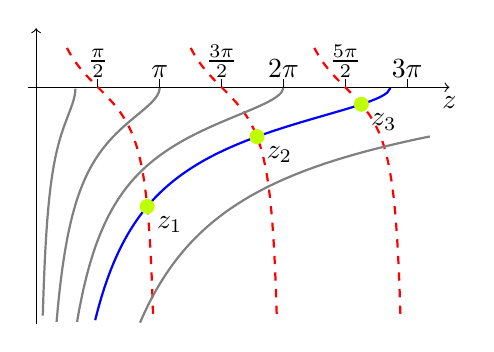
\begin{tikzpicture}[scale=0.5]
        % % region
        % \fill[lightgray] (-2,0) rectangle (0,3);
        % \fill[lightgray] (3,0) rectangle (5,2);
        % axis
        \draw[->] (-0.2,0) -- (10.5, 0);
        \draw[->] (0,-6) -- (0, 1.5);
        % text
        % \node[right] at (0,2) {I};
        \node[below] at (10.5,0) {$z$};
    
        \draw (pi/2,0) -- (pi/2,0.2);
        \node[above] at (pi/2,0) {$\frac{\pi}2$};
        \draw (pi,0) -- (pi,0.2);
        \node[above] at (pi,0) {$\pi$};
    
        \draw (3*pi/2,0) -- (3*pi/2,0.2);
        \node[above] at (3*pi/2,0) {$\frac{3\pi}2$};
        \draw (2*pi,0) -- (2*pi,0.2);
        \node[above] at (2*pi,0) {$2\pi$};
    
        \draw (5*pi/2,0) -- (5*pi/2,0.2);
        \node[above] at (5*pi/2,0) {$\frac{5\pi}2$};
        \draw (3*pi,0) -- (3*pi,0.2);
        \node[above] at (3*pi,0) {$3\pi$};
        % \node[above right ] at (0,2) {$V_0$};
        % functions
        \draw[domain=pi/4:pi-0.17,red,thick,dashed,samples=100] plot (\x,{cot(deg(\x))});
        \draw[domain=pi+pi/4:2*pi-0.17,red,thick,dashed,samples=100] plot (\x,{cot(deg(\x))});
        \draw[domain=2*pi+pi/4:3*pi-0.17,red,thick,dashed,samples=100] plot (\x,{cot(deg(\x))});
        
        \draw[domain=1.5:9,blue,thick,samples=100] plot (\x,{-sqrt(81/(\x*\x) - 1)});
        \draw[domain=0.17:1,gray,thick,samples=100] plot (\x,{-sqrt(1/(\x*\x) - 1)});
        \draw[domain=0.52:pi,gray,thick,samples=100] plot (\x,{-sqrt(pi*pi/(\x*\x) - 1)});
        \draw[domain=1.04:2*pi,gray,thick,samples=100] plot (\x,{-sqrt(4*pi*pi/(\x*\x) - 1)});
        \draw[domain=2.64:10,gray,thick,samples=100] plot (\x,{-sqrt(16*16/(\x*\x) - 1)});

        % roots
        \fill[draw, lime] (2.82259, -3.02769) circle[radius=5pt];
        \fill[draw, lime] (5.61016, -1.25442) circle[radius=5pt];
        \fill[draw, lime] (8.26182, -0.43206) circle[radius=5pt];
    
        \node[below right] at (2.82259, -3.02769) {$z_1$};
        \node[below right] at (5.61016, -1.25442) {$z_2$};
        \node[below right] at (8.26182, -0.43206) {$z_3$};
        
    \end{tikzpicture}
    \caption{半无限深势阱的解}
\end{figure}
当 $z_0 = 9$ 时,那么 $z$ 的取值是 $[0, z_0]$,画出图来看到只有 3 个解。对应于 3 个分离的束缚态 $E_i (i = 1, 2, 3)$,
\begin{eqnarray}
    E_i = \frac{\hbar^2 z^2}{2ml^2}, \quad i = 1, \cdots, N
\end{eqnarray}

最终给出半无限深势阱的波函数,
\begin{align}
    \psi_i (x) = 
    \begin{cases}
        0, \quad &x\in (-\infty, 0), \\
        C_1 \ee^{\ii k_2 x} - C_1 \ee^{-\ii k_2 x}, \quad &x\in[0,l],\\
        C_4 \ee^{-k_3 x}, \quad & x\in(l, \infty),
    \end{cases}
\end{align}
%2022-09-26 14:12:50  Wenbin Fan @FDU
% 将 $E_i$ 代入边界条件3中,得到
% \begin{align}
%     C_1 (\ee^{\ii k_2 l} - \ee^{-\ii k_2 l}) &= C_4 \ee^{-k_3 l}
% \end{align}
再给出\textbf{边界条件 5},波函数归一化
\begin{eqnarray}
    \intinf \psi^* \psi \, \dd x = 1,
\end{eqnarray}
由边界条件 3 \eqref{eq:half_condition_3} 和上式便可确定 $\{C_1, C_4\}$。边条件 3 中解得
\begin{equation}
    C_4 = C_1 \, 2\ii \,\ee^{k_3 l} \sin k_2 l,
\end{equation}
\begin{lstlisting}
Solve[Subscript[C, 1] (Exp[I k2 l] - Exp[-I k2 l]) == 
    Subscript[C, 4] Exp[-k3 l], Subscript[C, 4]] // 
  ExpToTrig // FullSimplify
>> {{Subscript[C, 4] -> 
   2 I E^(k3 l) Sin[k2 l] Subscript[C, 1]}}
\end{lstlisting}
由归一化条件可解得,
\begin{equation}
    C_1 = -\frac{\ii}2\left(
        \frac l2 + \frac1{2 k_3} \sin^2 k_2 l + \frac1{k_2} \sin 2k_2 l
    \right)^{-1/2}. 
\end{equation}
\begin{lstlisting}
res = Integrate[
    Subscript[C, 1] 2 I Sin[k2 x] Subscript[C, 1] 2 (- I) Sin[
        k2 x], {x, 0, l}] + 
    Integrate[
    2 I E^(k3 l) Sin[k2 l] Subscript[C, 1] Exp[-k3 x] 2 (-I) E^(k3 l)
        Sin[k2 l] Subscript[C, 1] Exp[-k3 x], {x, l, Infinity}, 
    Assumptions -> {k3 > 0}]
Solve[res == 1, Subscript[C, 1]] // FullSimplify
(* 运行结果略 *)
\end{lstlisting}

从以上 5 个边界条件,能给出量子化的条件。对于给定的 $z_0$ 能给出束缚态的解。

特别地,当 $z_0 < \pi/2$ 时,波函数将无解,不再有束缚态。不是只要有能垒就能束缚住电子。

% 2022-09-26 14:25:09  Wenbin Fan @FDU
% 第四节课
% 【画出波函数的图,拍照,黑、红、绿】

\boldtext{散射态}  $E > V_0$,解得
\begin{eqnarray}
    s^2 = \frac{(V_0 - E) 2 m}{\hbar^2} \rightarrow s = \pm \frac{\ii \sqrt{2m(E- V_0)}}{\hbar},
\end{eqnarray}
即
\begin{eqnarray}
    \psi(x) = C_3 \ee^{\ii k_3 x} + C_4 \ee^{-\ii k_3 x}, \quad k_3 = \frac{\ii\sqrt{2m(E-V_0)}}{\hbar},
\end{eqnarray}
这里有虚数,所以不能用无穷大的边界条件了。

\textbf{边界条件 3},
\begin{eqnarray}
    \psi(l^-) = \psi(l^+),
\end{eqnarray}
即
\begin{eqnarray}
    C_1 (\ee^{\ii k_2 l} - \ee^{-\ii k_2 l}) = 
    C_3 \ee^{\ii k_3 l} + C_4 \ee^{-\ii k_3 l}
\end{eqnarray}
\textbf{边界条件 4},
\begin{eqnarray}
    \psi'(l^-) = \psi'(l^+)
\end{eqnarray}
% 【检查上面的边界条件有没有 prime】
即
\begin{eqnarray}
    C_1 \ii k_2 (\ee^{\ii k_2 l} + \ee^{\ii k_2 l}) = \ii k_3 (C_3 \ee^{\ii k_3 l} - C_4 \ee^{-\ii k_3 l} )
\end{eqnarray}
省略推导过程,可以解出来
\begin{align}
    &C_3 = \frac12 \left[
        \left(1 + \frac{k_2}{k_3}\right) \ee^{\ii k_2 l} - 
        \left(1 - \frac{k_2}{k_3}\right) \ee^{-\ii k_2 l}
    \right] \ee^{-\ii k_3 l }C_1, \label{eq:half_inf_scat_c3}\\
    &C_4 = \frac12 \left[
        \left(1 - \frac{k_2}{k_3}\right) \ee^{\ii k_2 l} - 
        \left(1 + \frac{k_2}{k_3}\right) \ee^{-\ii k_2 l}
    \right] \ee^{\ii k_3 l} C_1, \label{eq:half_inf_scat_c4}
\end{align}
\begin{lstlisting}
Clear["Global`*"]
Solve[{Subscript[C, 1] (Exp[I k2 l] - Exp[-I k2 l]) == 
    Subscript[C, 3] Exp[I k3 l] + Subscript[C, 4] Exp[-I k3 l], 
    Subscript[C, 1] k2 (Exp[I k2 l] + Exp[-I k2 l]) == 
    k3 (Subscript[C, 3] Exp[I k3 l] - 
        Subscript[C, 4] Exp[-I k3 l])}, {Subscript[C, 3], 
    Subscript[C, 4]}] // FullSimplify
>> {{Subscript[C, 3] -> (
    E^(-I k3 l) (k2 Cos[k2 l] + I k3 Sin[k2 l]) Subscript[C, 1])/k3, 
    Subscript[C, 4] -> (
    E^(I k3 l) (-k2 Cos[k2 l] + I k3 Sin[k2 l]) Subscript[C, 1])/k3}}
\end{lstlisting}
%2022-09-26 14:34:13  Wenbin Fan @FDU

有几个结论,
(1) 注意到 $C_3^* = C_4$,可以知道 $\psi(x)$ 在 block III 是实三角函数,
(2) $k_2$ 与 $k_3(E)$ 没有任何限制要求,即本征值无限多,散射态是连续谱。因为没有其它可用的边界条件了,所以没有了量子化的能级。尽管这有点违背直觉。

\homework{
    \textbf{3.4}
    (1) 利用公式 \eqref{eq:half_inf_scat_c4},求
    $|C_1|^2$ 与 $|C_3|^2$ 
     的关系,并比较二者大小。
}

散射态的方程为
\begin{eqnarray}
    \phi (x) = \begin{cases}
        0, \quad &x \in (-\infty, 0), \\
        C_1 \ee^{\ii k_2 x} - C_1 \ee^{-\ii k_2 x}, \quad &x \in [0,l], \\
        C_3 \ee^{\ii k_3 x} + C_4 \ee^{-\ii k_3 x}, \quad &x \in (l, \infty),
    \end{cases}
\end{eqnarray}
直觉上来理解,$|C_1|^2$ 是粒子散射态反射回来的概率,$|C_3|^2$ 是投射过去的概率。

\homework{
    \textbf{3.4} (2) 推导并画出 $z = 12$, $z_0 = 9$ 时的体系波函数。
}

\section{阶梯势垒体系}
\begin{figure}[tp]\centering
    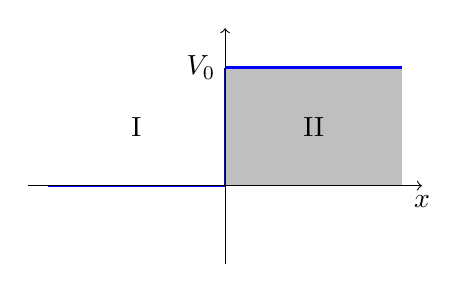
\begin{tikzpicture}[scale=0.5]
        % region
        % \fill[lightgray] (-5,0) rectangle (0,4);
        \fill[lightgray] (0,0) rectangle (4.5,3);
        \draw[blue,thick] (-4.5,0) -- (0,0);
        \draw[blue,thick] (0,0) -- (0,3);
        \draw[blue,thick] (0,3) -- (4.5,3);
        % axis
        \draw[->] (-5,0) -- (5, 0);
        \draw[->] (0,-2) -- (0, 4);
        % text
        \node[below] at (5,0) {$x$};
        \node[left] at (0,3) {$V_0$};
        \node at (-2.25, 1.5) {I};
        \node at (2.25, 1.5) {II};
    \end{tikzpicture}
\caption{阶梯势垒}
\end{figure}
\begin{eqnarray}
    V(x) = 
\begin{cases}
    0, \quad x\in(-\infty, 0), \\
    V_0, \quad x\in[0, \infty],
\end{cases}
\end{eqnarray}

对于 block I, 解出
\begin{eqnarray}
    \psi(x) = C_1 \ee^{\ii k_1 x} + C_2 \ee^{- \ii k_2 x},
\end{eqnarray}
其中
\begin{eqnarray}
    k_1 = \frac{\sqrt{2mE}}{\hbar}
\end{eqnarray}
有三个待定参数 $\{C_1, C_2, E\}$。

对于 block II,与单侧无限深势阱中的 block III 是一致的。
% 【直接复制过来上面的求解,已拍照】
%2022-09-26 14:46:05  Wenbin Fan @FDU

\boldtext{散射态} $E > V_0$,推出
\begin{eqnarray}
    S = \pm \ii k_2, \quad k_2 = \frac{\sqrt{2m(E-V_0)}}{\hbar}
\end{eqnarray}
波函数
\begin{align}
    \psi(x) = \begin{cases}
        C_1 \ee^{\ii k_1 x} + C_2 \ee^{\ii k_1 x},\quad & x \in (-\infty, 0), \\
        C_3 \ee^{\ii k_2 x} + C_4 \ee^{\ii k_2 x}, \quad & x \in [0, \infty),
    \end{cases}
\end{align}
有 5 个待定参数 $\{C_1, C_2, C_3, C_4, E\}$。

% 【画图】
多个动量本征态的叠加。
% $C_1$ $C_3$ 都是向右方向的动量本征矢。
\begin{figure}[tp]\centering
    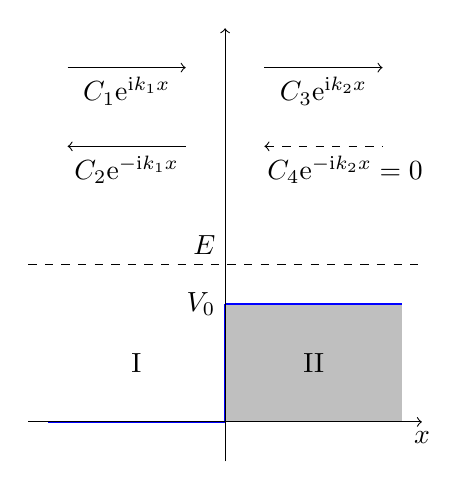
\begin{tikzpicture}[scale=0.5]
        % region
        % \fill[lightgray] (-5,0) rectangle (0,4);
        \fill[lightgray] (0,0) rectangle (4.5,3);
        \draw[blue,thick] (-4.5,0) -- (0,0);
        \draw[blue,thick] (0,0) -- (0,3);
        \draw[blue,thick] (0,3) -- (4.5,3);
        % axis
        \draw[->] (-5,0) -- (5, 0);
        \draw[->] (0,-1) -- (0, 10);
        % text
        \node[below] at (5,0) {$x$};
        \node[left] at (0,3) {$V_0$};
        \node at (-2.25, 1.5) {I};
        \node at (2.25, 1.5) {II};
        %
        \draw[dashed] (-5, 4) -- (5, 4);
        \node[above left] at (0,4) {$E$};
        %
        \draw[->] (-4,9) -- (-1,9);
        \node[below] at (-2.5, 9) {$C_1 \mathrm{e}^{\mathrm ik_1 x}$};
        \draw[<-] (-4,7) -- (-1,7);
        \node[below] at (-2.5, 7) {$C_2 \mathrm{e}^{-\mathrm ik_1 x}$};
        \draw[->] (1,9) -- (4,9);
        \node[below] at (2.5, 9) {$C_3 \mathrm{e}^{\mathrm ik_2 x}$};
        \draw[<-,dashed] (1,7) -- (4,7);
        \node[below] at (2.5, 7) {$\phantom{0=}C_4 \mathrm{e}^{-\mathrm ik_2 x} = 0$};
    
        % functions
        % \draw[domain=pi/4:pi-0.17,red,thick,dashed,samples=100] plot (\x,{cot(deg(\x))});
    \end{tikzpicture}
    \caption{波的方向示意图}
\end{figure}

概率流密度的定义
\begin{eqnarray}
    J = \frac{\ii\hbar}{2m} \left[
        \psi^* \pdv[x] \psi - \psi \pdv[x] \psi^*
    \right]
\end{eqnarray}
对于 block I,
\begin{eqnarray}
    J_1 = \frac{k_1 \hbar}{m} \left(
        |C_1|^2 - |C_2|^2
    \right)
\end{eqnarray}
这个体系中的截面只有一条线,流入为负,流出为正,因此
$\frac{k_1 \hbar}{m} |C_1|^2$ 为进入 block I 入射波($C_1 \ee^{-\ii k_1 x}$)的概率流密度,
同理 $\frac{k_1 \hbar}{m} |C_2|^2$ 为反射波($C_2 \ee^{-\ii k_2 x}$)的概率流密度,因此可得 $\frac{k_2 \hbar}{m} |C_3|^2$ 为进入 block III 的波($C_3 \ee^{\ii k_3 x}$)的概率流密度,特别地,$\frac{k_2 \hbar}{m} |C_4|^2 = 0$,因为不会有反射回来的波,所以 $C_4 = 0$。

思考,一个能量为 $E$($E>V_0$)的粒子从 $\infty$ 向 $-\infty$ 传播,此时边界条件 3
\begin{eqnarray}
    \psi(0^-) = \psi(0^+),
\end{eqnarray}
推出
\begin{eqnarray}
    C_1 + C_2 = C_3,
\end{eqnarray}
边界条件 4
\begin{eqnarray}
    \psi'(0^-) = \psi'(0^+)
\end{eqnarray}
推出
\begin{eqnarray}
    k_1 (C_1 - C_2) = k_2 C_3,
\end{eqnarray}
联立解得
% 【见照片,有 ref】
%2022-09-26 15:02:08  Wenbin Fan @FDU
% 【k1 k2 def】【没拍全】
\begin{align}
    & C_2 = \frac{k_1 - k_2} {k_1 + k_2} C_1, \\
    & C_3 = \frac{k_1}{k_1 + k_2} C_1,
\end{align}

定义反射系数
\begin{eqnarray}
    R = \frac{ \displaystyle \frac{k_1 h}m |C_2|^2 } { \displaystyle \frac{k_1 h}m |C_1|^2 } = \frac{(k_1 - k_2)^2} {(k_1 + k_2)^2}, 
\end{eqnarray}
定义透射系数,
\begin{eqnarray}
    T = \frac{ \displaystyle \frac{k_2 h}m |C_2|^2 } { \displaystyle \frac{k_1 h}m |C_1|^2 } = \frac{4k_1k_2} {(k_1 + k_2)^2}, 
\end{eqnarray}
显然有 $R^2 + T^2 = 1$。

代入 $k_1, k_2$ 的定义
\begin{eqnarray}
    R = \left( 1 - \sqrt{1 - \frac{V_0}E}\right)^2 
    \left( 1 + \sqrt{1 - \frac{V_0}E}\right)^{-2},
\end{eqnarray}
当 $0 < \frac{V_0}{E} < 1$ 时,
% 【画图 R - (V0/E) 的图,类似 $x^2$ 的图】
哪怕到了 $\frac{V_0}E = 80\%$,透射率只有 15\%,当 $E = V_0$ 时全反射,并不是像想象中的那样越过去。
\begin{lstlisting}
(* 画出 R-(V0/E) 的图 *)
Plot[(-1 + Sqrt[1 - x])^2/(1 + Sqrt[1 - x])^2, {x, 0, 1}, 
    PlotRange -> {0, 1}]
\end{lstlisting}

\section{有限高方势垒}
\begin{figure}[tp]\centering
    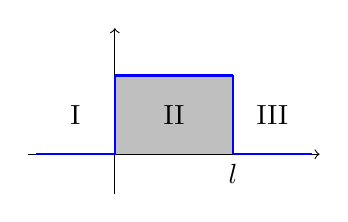
\begin{tikzpicture}[scale=0.5]
        % \fill[lightgray] (-2,0) rectangle (0,3);
        \fill[lightgray] (0,0) rectangle (3,2);
        % axis
        \draw[->] (-2.2,0) -- (5.2, 0);
        \draw[->] (0,-1) -- (0, 3.2);
        % potential
        \draw[thick,blue] (-2,0) -- (0,0);
        \draw[thick,blue] (0,0) -- (0,2);
        \draw[thick,blue] (0,2) -- (3,2);
        \draw[thick,blue] (3,0) -- (3,2); 
        \draw[thick,blue] (3,0) -- (5,0);
        % text
        \node[] at (-1,1) {I};
        \node[] at (1.5,1) {II};
        \node[] at (4,1) {III};
        
        \node[below] at (3,0) {$l$};
        % functions
        % \draw[domain=pi/4:pi-0.17,red,thick,dashed,samples=100] plot (\x,{cot(deg(\x))});
    \end{tikzpicture}
    \caption{有限高方势垒}
    \end{figure}
势能的形式,
\begin{eqnarray}
    V(x) = 
        \begin{cases}
            0, \quad &x \in (-\infty,0),\\
            V_0, \quad &x \in[0,l],\\
            0, \quad &x \in (l, \infty),
        \end{cases}
\end{eqnarray}

分情况讨论,$E<V_0$ 时,得到波函数
\begin{eqnarray}
    \psi(x) =
\begin{cases}
    C_1 \ee^{\ii k_1 x} + C_2 \ee^{-\ii k_1 x}, \quad &x \in (-\infty, 0), \\
    C_3 \ee^{\ii k_2 x} + C_4 \ee^{-k_2 x}, \quad &x \in[0,l],\\
    C_5 \ee^{\ii k_3 x}, \quad &x \in(l, \infty),
\end{cases}
\end{eqnarray}
\homework{
    \textbf{3.5} 求出有限高方势垒($E<V_0$)的波函数。
}